\documentclass[xcolor={table}]{beamer}
\usepackage{fleqn}
\usepackage{graphicx}
\usepackage{coordsys} %for \numbline commander

%Setup appearance:
\usetheme{Darmstadt}
\usefonttheme[onlylarge]{structurebold}
\setbeamerfont*{frametitle}{size=\normalsize,series=\bfseries}
\setbeamertemplate{navigation symbols}{}
\setbeamertemplate{bibliography item}{[\theenumiv]}

% Standard packages
\usepackage[english]{babel}
\usepackage[latin1]{inputenc}
\usepackage{times}
\usepackage[T1]{fontenc}
\usepackage{multirow}
\usepackage{subfigure}
\usepackage{pbox}
\usepackage{arydshln}
\usepackage{pifont}
\usepackage{cancel}
\usepackage{rotating} % for sideways headings

% Source Code packages
\usepackage{algorithm2e}
\usepackage{algorithmic}

\DeclareSymbolFont{extraup}{U}{zavm}{m}{n}
\DeclareMathSymbol{\varclub}{\mathalpha}{extraup}{84}
\DeclareMathSymbol{\varspade}{\mathalpha}{extraup}{85}
\DeclareMathSymbol{\varheart}{\mathalpha}{extraup}{86}
\DeclareMathSymbol{\vardiamond}{\mathalpha}{extraup}{87}

%%% This section command that adds a big page with section dividers
\usepackage{xifthen}% provides \isempty test
\newcommand{\SectionSlide}[2][]{
	\ifthenelse{\isempty{#1}}
		{\section{#2}\begin{frame} \begin{center}\begin{huge}#2\end{huge}\end{center}\end{frame}}
		{\section[#1]{#2}\begin{frame} \begin{center}\begin{huge}#2\end{huge}\end{center}\end{frame}}
}
%Extends the section slide to to include a shortened section title for the navigation bar as a second parameter
\newcommand{\SectionSlideShortHeader}[3][]{
	\ifthenelse{\isempty{#1}}
		{\section[#3]{#2}\begin{frame} \begin{center}\begin{huge}#2\end{huge}\end{center}\end{frame}}
		{\section[#1]{#2}\begin{frame} \begin{center}\begin{huge}#3\end{huge}\end{center}\end{frame}}
}

\newcommand{\refer}[1]{\footnote{#1}}
\newcommand{\GW}{\text{\textit{Guess-Who~}}}
\newcommand{\keyword}[1]{\alert{\textbf{#1}}\index{#1}}
\newcommand{\firstkeyword}[1]{\textbf{#1}\index{#1}}
\newcommand{\indexkeyword}[1]{\alert{\textbf{#1}\index{#1}}}
\newcommand{\featN}[1]{\textsc{#1}}
\newcommand{\featL}[1]{\textit{'#1'}}
 \newcommand{\ourRef}[1]{\ref{#1} $^{\text{\tiny[\pageref{#1}]}}$}
 \newcommand{\ourEqRef}[1]{\eqref{#1}$^{\text{\tiny[\pageref{#1}]}}$}
  
\DeclareMathOperator*{\argmax}{argmax}
\DeclareMathOperator*{\argmin}{argmin}



\title{Similarity-based Learning\\Sections $5.1, 5.2, 5.3$}
	\author{John D. Kelleher and Brian Mac Namee and Aoife D'Arcy}
	\institute{}
	\date{}

\begin{document}
\begin{frame}
	\titlepage
\end{frame}
\begin{frame}
	 \tableofcontents
\end{frame}

\SectionSlide{Big Idea}

\begin{frame} 
\begin{itemize}
\item The year is 1798 and you are Lieutenant-Colonel David Collins of HMS Calcutta who is exploring the region around Hawkesbury River, in New South Wales. 
\item After an expedition up the river one of the men tells you that he saw a strange animal near the river.  
\item You ask him to describe the animal to you and he explains that he didn't see it very well but that he did notice that it had webbed feet and a duck-bill snout, and that it growled at him.
\item In order to plan the expedition for the next day you decide that you need to classify the animal so that you can figure out whether it is dangerous to approach it or not.  
\end{itemize}
\end{frame} 

 \begin{frame} [plain]
\begin{figure}[htb]
	\begin{center}
\resizebox{0.75\textwidth}{!}{\begin{tabular}{c | c c c | c}
~ & \Large{\textit{Grrrh!}} & 
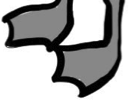
\includegraphics[width=0.08\textwidth]{./images/DuckLegs.png}&

\includegraphics[width=0.08\textwidth]{./images/DuckBeak.png}&
\textbf{Score} \\
\hline
~&
~ &
~ &
~ &
~\\
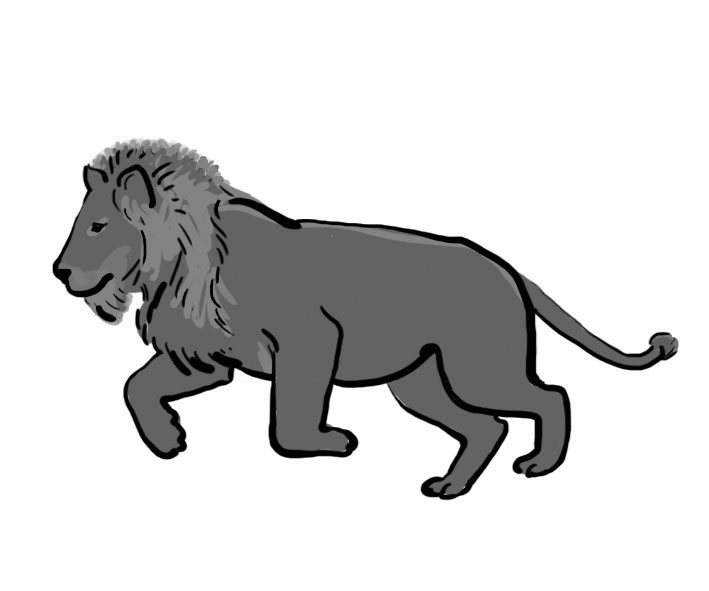
\includegraphics[width=0.15\textwidth]{./images/LionBW.png}&
\Huge{\ding{51}} &
\Huge{\ding{55}} &
\Huge{\ding{55}} &
\Huge{1}\\
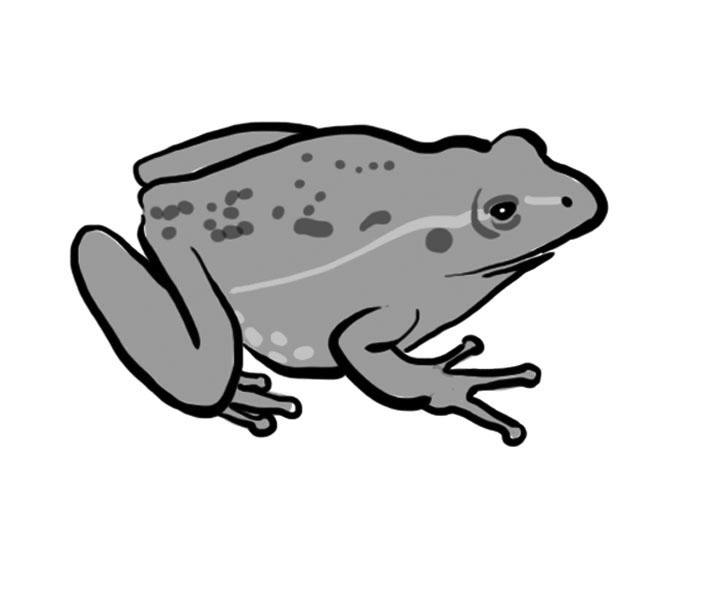
\includegraphics[width=0.15\textwidth]{./images/FrogBW.png}&
\Huge{\ding{55}} &
\Huge{\ding{51}} &
\Huge{\ding{55}} &
\Huge{1}\\
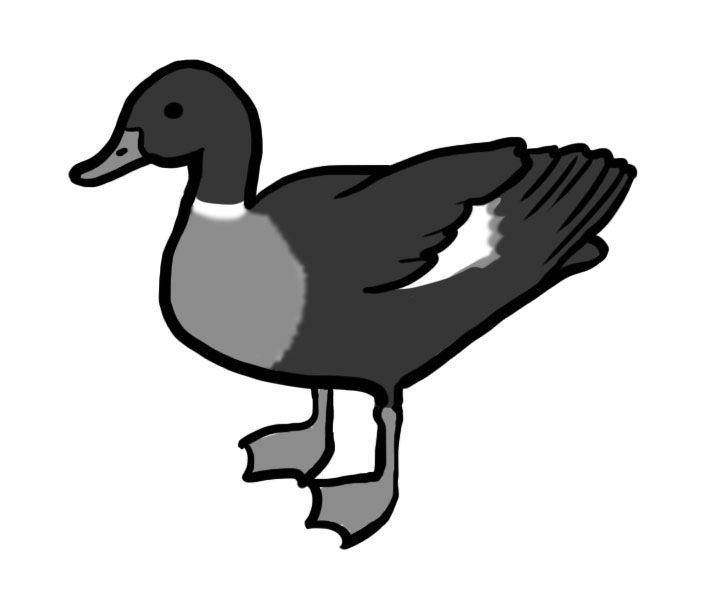
\includegraphics[width=0.15\textwidth]{./images/DuckBW.png}&
\Huge{\ding{55}} &
\Huge{\ding{51}} &
\Huge{\ding{51}} &
\Huge{2}\\
	\end{tabular}}
	\end{center}
       \caption{Matching animals you remember to the features of the unknown animal described by the sailor. Note: The images used in this figure were created by Jan Gillbank for the English for the Australian Curriculum website (\url{http://www.e4ac.edu.au}) and are used under the Create Commons Attribution 3.0 Unported licence (\url{http://creativecommons.org/licenses/by/3.0}). The images were sourced via Wikimedia Commons.}	
	\label{fig:animalFeatureMatching}
\end{figure}
\end{frame} 

\begin{frame} 
\begin{itemize}
\item The process of classifying an unknown animal by matching the features of the animal against the features of animals you can remember neatly encapsulates the big idea underpinning similarity-based learning: 

\begin{center} 

~\\

\textit{if you are trying to classify something then you should search your memory to find things that are similar and label it with the same class as the most similar thing in your memory}

~\\

\end{center}

\item One of the simplest and best known machine learning algorithms for this type of reasoning is called the \alert{nearest neighbor} algorithm. 
\end{itemize}
\end{frame} 


\SectionSlide{Fundamentals}

\begin{frame} 
\begin{itemize}
\item The fundamentals of similarity-based learning are:
\begin{itemize}
\item Feature space
\item Similarity metrics
\end{itemize}
\end{itemize}
\end{frame} 


\subsection{Feature Space}



 \begin{frame} 
\begin{table}[htb]
\caption{The speed and agility ratings for 20 college athletes labelled with the decisions for whether they were drafted or not. }
\label{table:draftProspects}
\begin{footnotesize}
\centering
\begin{tabular}{cc}
		\hline
			\begin{minipage}{0.45\textwidth}
\centering
					\begin{tabular}[ht]{cccc} 
\textbf{ID}	 & \textbf{Speed} & \textbf{Agility} & \textbf{Draft}\\
\hline
1 & 2.50 & 6.00 & No\\
2 & 3.75 & 8.00 & No\\
3 & 2.25 & 5.50 & No\\
4 & 3.25 & 8.25 & No\\
5 & 2.75 & 7.50 & No\\
6 & 4.50 & 5.00 & No\\
7 & 3.50 & 5.25 & No\\
8 & 3.00 & 3.25 & No\\
9 & 4.00 & 4.00 & No\\
10 & 4.25 & 3.75 & No\\
\hline
					\end{tabular}
			\end{minipage}
			&
			\begin{minipage}{0.45\textwidth}
\centering
					\begin{tabular}[ht]{cccc} 
\textbf{ID}	 & \textbf{Speed} & \textbf{Agility} & \textbf{Draft}\\
\hline
11 & 2.00 & 2.00 & No\\
12 & 5.00 & 2.50 & No\\
13 & 8.25 & 8.50 & No\\
14 & 5.75 & 8.75 & Yes\\
15 & 4.75 & 6.25 & Yes\\
16 & 5.50 & 6.75 & Yes\\
17 & 5.25 & 9.50 & Yes\\
18 & 7.00 & 4.25 & Yes\\
19 & 7.50 & 8.00 & Yes\\
20 & 7.25 & 5.75 & Yes\\
\hline
				\end{tabular}
			\end{minipage}\\
\end{tabular}
\end{footnotesize}
\end{table}
\end{frame} 



 \begin{frame} [plain]
\begin{figure}[htb]
       \begin{centering}
       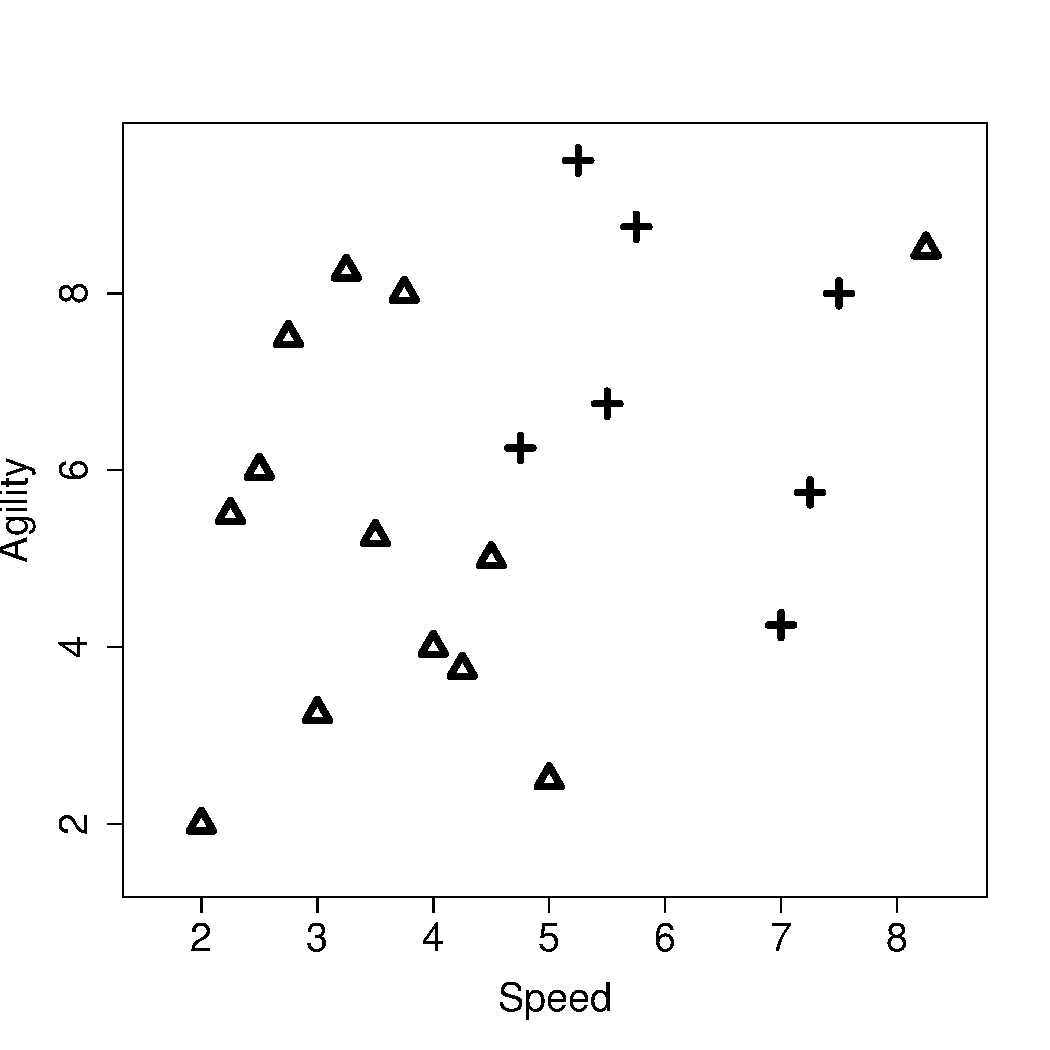
\includegraphics[width=0.7\textwidth]{images/knn_fs_1.pdf}
       \caption{A feature space plot of the  data in Table \ourRef{table:draftProspects}. The  triangles represent \featL{Non-draft} instances and the crosses represent the \featL{Draft} instances.}
       \label{fig:featurespace}
       \end{centering}
\end{figure}
\end{frame} 

\begin{frame} 
\begin{itemize}
\item A \alert{feature space} is an abstract n-dimensional space that is created by taking each of the descriptive features in an ABT to be the axes of a reference space and each instance in the dataset is mapped to a point in the feature space based on the values of its descriptive features. 
\end{itemize}
\end{frame} 



\subsection{Distance Metrics}

\begin{frame}
\begin{itemize}
\item A \alert{similarity metric} measures the similarity between two instances according to a feature space
\item Mathematically, a \alert{metric} must conform to the following four criteria:
\begin{enumerate}
	\item \alert{Non-negativity}: $metric(\textbf{a},\textbf{b}) \geq 0$
	\item \alert{Identity}: $metric(\textbf{a},\textbf{b}) = 0 \Longleftrightarrow \textbf{a}=\textbf{b}$ 
	\item \alert{Symmetry}: $metric(\textbf{a},\textbf{b}) = metric(\textbf{b},\textbf{a})$
	\item \alert{Triangular Inequality}: $metric(\textbf{a},\textbf{b}) \leq metric(\textbf{a},\textbf{c}) + metric(\textbf{b},\textbf{c})$
\end{enumerate}

where $metric(\textbf{a},\textbf{b})$ is a function that returns the distance between two instances $\textbf{a}$ and $\textbf{b}$.
\end{itemize}
\end{frame} 

 \begin{frame} 
 \begin{itemize}
\item One of the best known metrics is \alert{Euclidean distance} which computes the length of the straight line between two points. Euclidean distance between two instances $\textbf{a}$ and $\textbf{b}$ in a $m$-dimensional feature space is defined as: 

~~\\

\begin{equation}
Euclidean(\textbf{a},\textbf{b}) = \sqrt{\sum_{i=1}^{m} \left(\textbf{a}[i] - \textbf{b}[i]\right)^2}
\label{eq:euclid}
\end{equation}
\end{itemize}
\end{frame} 



 \begin{frame} 
 \begin{example} 
The Euclidean distance between instances $d_{12}$ (\featN{Speed}$= 5.00$, \featN{Agility}$=2.5$) and $d_5$ (\featN{Speed}$=2.75$,\featN{Agility}$=7.5$) in Table \ourRef{table:draftProspects} is:
 
  \begin{overprint}
		  \onslide<1>
            \onslide<2>
             \begin{equation*}
			\footnotesize
			\begin{alignedat}{2}
			Euclidean(\left<5.00,2.50\right>,\left<2.75,7.50\right>) &= 
			\sqrt{\left( 5.00 - 2.75\right )^2 + \left( 2.50 - 7.50 \right)^2}\\
			& = \sqrt{30.0625}=5.4829
			\end{alignedat}
			\label{eq:euclidexample}
		\end{equation*}
\end{overprint}
        

\end{example} 
\end{frame} 

 \begin{frame} 
\begin{itemize}
\item Another, less well known, distance measure is the \alert{Manhattan} distance or \alert{taxi-cab distance}. 
\item The Manhattan distance between two instances $\textbf{a}$ and $\textbf{b}$ in a feature space with $m$ dimensions is:\footnote{The $abs()$ function surrounding the subtraction term indicates that we use the absolute value, i.e. non-negative value, when we are summing the differences; this makes sense because distances can't be negative.}
 
\begin{equation}
Manhattan(\textbf{a},\textbf{b}) = \sum_{i=1}^{m} abs(\textbf{a}[i] - \textbf{b}[i])
\label{eq:taxi}
\end{equation}

\end{itemize}
\end{frame} 



 \begin{frame} 
\begin{figure}[htb]
       \begin{centering}
       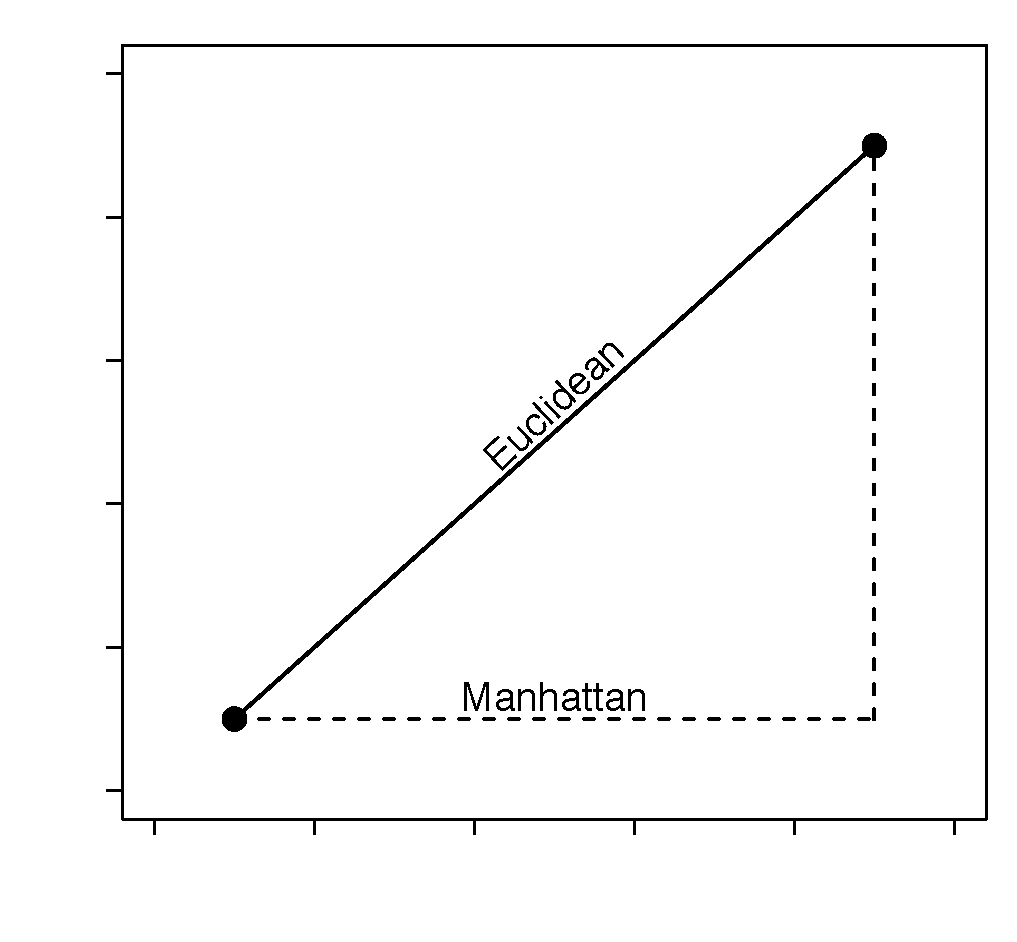
\includegraphics[width=0.65\textwidth]{images/manhattan_euclidean_1.pdf}
       \caption{The Manhattan and Euclidean distances between two points.}
       \label{fig:maneuc}
       \end{centering}
\end{figure}
\end{frame} 


 \begin{frame} 
 \begin{example} 
The Manhattan distance between instances $d_{12}$ (\featN{Speed}$= 5.00$, \featN{Agility}$=2.5$) and $d_5$ (\featN{Speed}$=2.75$,\featN{Agility}$=7.5$) in Table \ourRef{table:draftProspects} is:

\begin{overprint}
		  \onslide<1>
            \onslide<2>
\begin{equation*}
\footnotesize
	\begin{alignedat}{2}
Manhattan(\left<5.00,2.50\right>,\left<2.75,7.50\right>) &= abs( 5.00 - 2.75) + abs( 2.5 - 7.5)\\
& = 2.25 + 5= 7.25
	\end{alignedat}
\label{eq:manhattanexample}
\end{equation*}
\end{overprint}

\end{example} 
\end{frame} 


\begin{frame} 
\begin{itemize}
\item The Euclidean and Manhattan distances are special cases of \alert{Minkowski distance}
\item The \alert{Minkowski distance} between two instances $\textbf{a}$ and $\textbf{b}$ in a feature space with $m$ descriptive features is:

\begin{equation}
Minkowski(\textbf{a},\textbf{b}) = \left(\sum_{i=1}^{m} abs(\textbf{a}[i] - \textbf{b}[i])^{p}\right)^{\frac{1}{p}}
\label{eq:mink}
\end{equation}

where different values of the parameter $p$ result in different distance metrics
\item The Minkowski distance with $p=1$ is the Manhattan distance and with $p=2$ is the Euclidean distance.
\end{itemize}
\end{frame} 


\begin{frame} 
	\begin{itemize}
		\item The larger the value of $p$ the more emphasis is placed on the features with large differences in values because these differences are raised to the power of $p$. 
	\end{itemize}
\end{frame} 

       
\begin{frame} [plain]
	\begin{example}
		\centering
		\begin{footnotesize}
			\begin{tabular}{c c  c  c }
			\hline
			 & & \textbf{Manhattan} & \textbf{Euclidean}\\
			\textbf{Instance ID} & \textbf{Instance ID} & \textbf{(Minkowski p=1)} & \textbf{(Minkowski p=2)}\\
			\hline
			$12$ & $5$ & 7.25 & 5.4829	 \\
			$12$ & $17$ & 7.25 & 8.25 \\
			\hline
			\end{tabular}
		\end{footnotesize}
			
       	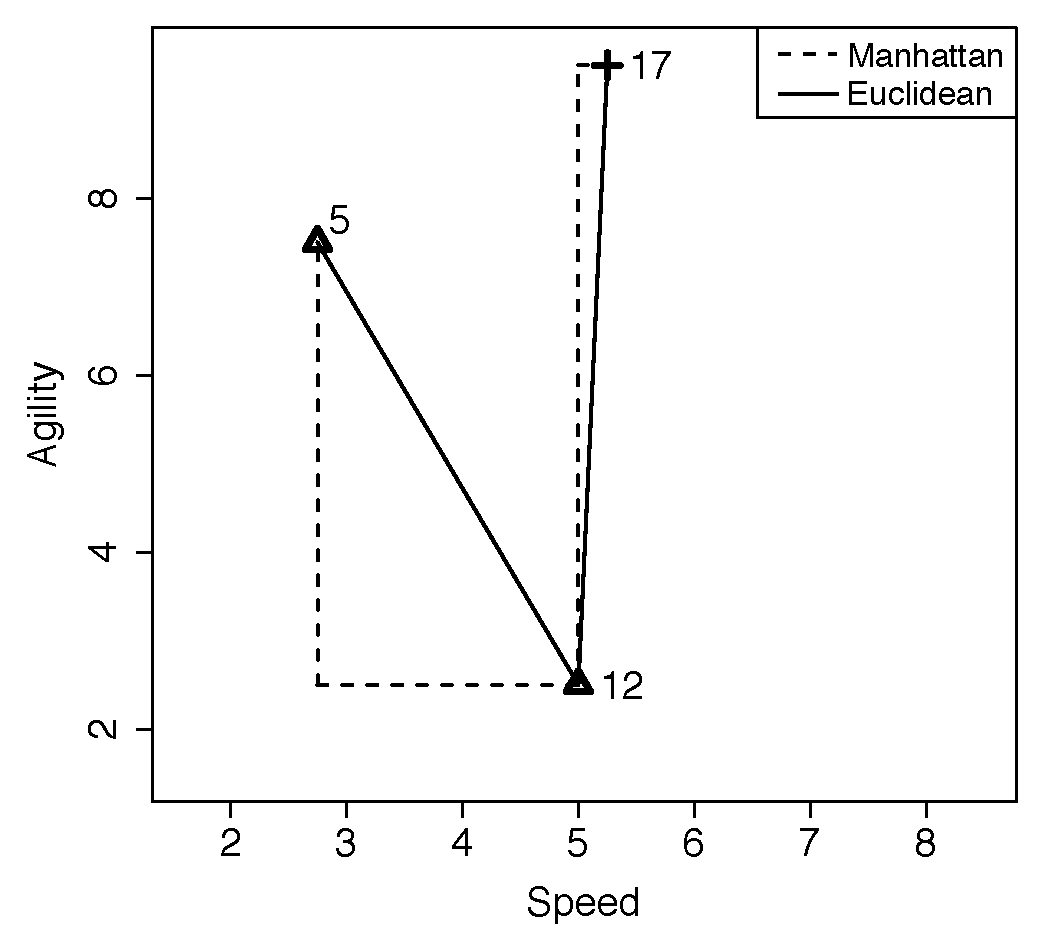
\includegraphics[width=0.5\textwidth]{images/manhattan_euclidean_2.pdf}
    		
			
			\footnotesize The Manhattan and Euclidean distances between instances $\mathbf{d}_{12}$ (\featN{Speed}$= 5.00$, \featN{Agility}$=2.5$) and $\mathbf{d}_{5}$ (\featN{Speed}$=2.75$, \featN{Agility}$=7.5$) and between instances $\mathbf{d}_{12}$ and $\mathbf{d}_{17}$ (\featN{Speed}$=5.25$, \featN{Agility}$=9.5$).
	\end{example}
\end{frame} 

\SectionSlideShortHeader{Standard Approach: The Nearest Neighbor Algorithm}{Standard Approach}

\begin{frame}
\begin{center} \textbf{The Nearest Neighbour Algorithm} \end{center}
\begin{algorithmic}[1]
\REQUIRE set of training instances
\REQUIRE a query to be classified
\\
\STATE Iterate across the instances in memory and find the instance that is shortest distance from the query position in the feature space.
\STATE Make a prediction for the query equal to the value of the target feature of the nearest neighbor.
\end{algorithmic}

~ \\

\end{frame}

\subsection{A Worked Example}

\begin{frame} 
\begin{table}[htb]
\caption{The speed and agility ratings for 20 college athletes labelled with the decisions for whether they were drafted or not. }
\label{table:draftProspects}
\begin{footnotesize}
\centering
\begin{tabular}{cc}
		\hline
			\begin{minipage}{0.45\textwidth}
\centering
					\begin{tabular}[ht]{cccc} 
\textbf{ID}	 & \textbf{Speed} & \textbf{Agility} & \textbf{Draft}\\
\hline
1 & 2.50 & 6.00 & No\\
2 & 3.75 & 8.00 & No\\
3 & 2.25 & 5.50 & No\\
4 & 3.25 & 8.25 & No\\
5 & 2.75 & 7.50 & No\\
6 & 4.50 & 5.00 & No\\
7 & 3.50 & 5.25 & No\\
8 & 3.00 & 3.25 & No\\
9 & 4.00 & 4.00 & No\\
10 & 4.25 & 3.75 & No\\
\hline
					\end{tabular}
			\end{minipage}
			&
			\begin{minipage}{0.45\textwidth}
\centering
					\begin{tabular}[ht]{cccc} 
\textbf{ID}	 & \textbf{Speed} & \textbf{Agility} & \textbf{Draft}\\
\hline
11 & 2.00 & 2.00 & No\\
12 & 5.00 & 2.50 & No\\
13 & 8.25 & 8.50 & No\\
14 & 5.75 & 8.75 & Yes\\
15 & 4.75 & 6.25 & Yes\\
16 & 5.50 & 6.75 & Yes\\
17 & 5.25 & 9.50 & Yes\\
18 & 7.00 & 4.25 & Yes\\
19 & 7.50 & 8.00 & Yes\\
20 & 7.25 & 5.75 & Yes\\
\hline
				\end{tabular}
			\end{minipage}\\
\end{tabular}
\end{footnotesize}
\end{table}
\end{frame} 

\begin{frame}
\begin{example}
\begin{itemize}
	\item Should we draft an athlete with the following profile:
\end{itemize}
	\begin{center}
	 \featN{Speed}$=6.75$, \featN{Agility}$=3$
	 \end{center}
	 \end{example}
\end{frame}

 \begin{frame} 
\begin{figure}[htb]
       \begin{centering}
       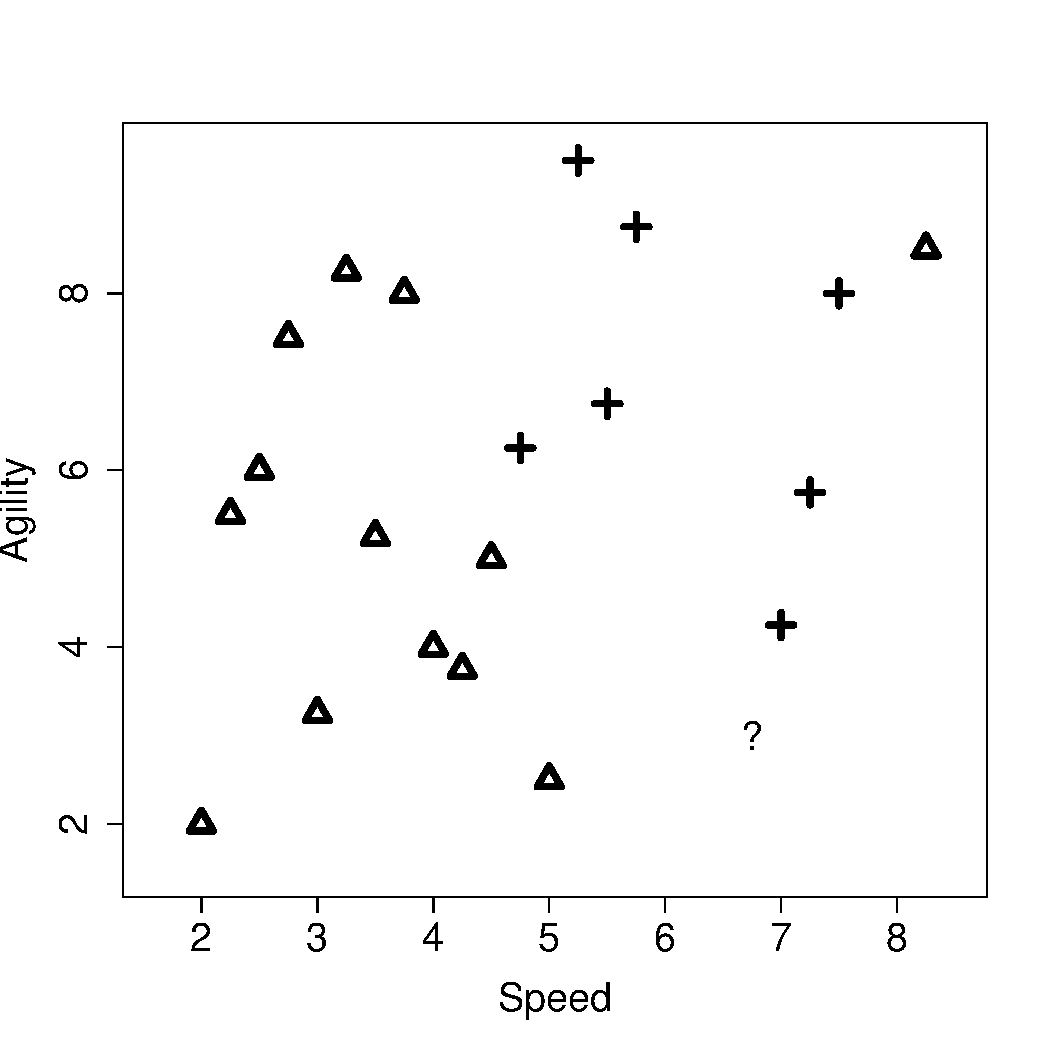
\includegraphics[width=0.5\textwidth]{images/knn_fs_2.pdf}
       \caption{A feature space plot of the  data in Table \ourRef{table:draftProspects} with the position in the feature space of the query represented by the ? marker. The  triangles represent \featL{Non-draft} instances and the crosses represent the \featL{Draft} instances.}
       \label{fig:queryfeaturespace}
       \end{centering}
\end{figure}
\end{frame} 

 \begin{frame} 
\begin{table}[htb]
\caption{The distances (Dist.) between the query instance with \featN{Speed}$\;=6.75$ and \featN{Agility}$\;=3.00$ and each instance in Table \ourRef{table:draftProspects}.}
\label{table:draftProspectsDistances}
\begin{tiny}
\begin{center}
\resizebox{\textwidth}{!}{\begin{tabular}{cc}
		\hline
			\begin{minipage}{0.45\textwidth}
					\begin{tabular}[ht]{ccccc} 
\featN{ID}	 & \featN{Speed} & \featN{Agility} & \featN{Draft} & Dist.\\
\hline
18	&	7.00	&	4.25	&	yes	&	1.27	\\
12	&	5.00	&	2.50	&	no	&	1.82	\\
10	&	4.25	&	3.75	&	no	&	2.61	\\
20	&	7.25	&	5.75	&	yes	&	2.80	\\
9	&	4.00	&	4.00	&	no	&	2.93	\\
6	&	4.50	&	5.00	&	no	&	3.01	\\
8	&	3.00	&	3.25	&	no	&	3.76	\\
15	&	4.75	&	6.25	&	yes	&	3.82	\\
7	&	3.50	&	5.25	&	no	&	3.95	\\
16	&	5.50	&	6.75	&	yes	&	3.95	\\
\hline
					\end{tabular}
			\end{minipage}
			&
			\begin{minipage}{0.45\textwidth}
					\begin{tabular}[ht]{ccccc} 
\featN{ID}	 & \featN{Speed} & \featN{Agility} & \featN{Draft} & Dist.\\
\hline
11	&	2.00	&	2.00	&	no	&	4.85	\\
19	&	7.50	&	8.00	&	yes	&	5.06	\\
3	&	2.25	&	5.50	&	no	&	5.15	\\
1	&	2.50	&	6.00	&	no	&	5.20	\\
13	&	8.25	&	8.50	&	no	&	5.70	\\
2	&	3.75	&	8.00	&	no	&	5.83	\\
14	&	5.75	&	8.75	&	yes	&	5.84	\\
5	&	2.75	&	7.50	&	no	&	6.02	\\
4	&	3.25	&	8.25	&	no	&	6.31	\\
17	&	5.25	&	9.50	&	yes	&	6.67	\\
\hline
				\end{tabular}
			\end{minipage}\\
\end{tabular}}
\end{center}
\end{tiny}
\end{table}
\end{frame} 



 \begin{frame} 
\begin{figure}[htb]
	\begin{centering}
\begin{tabular}{cc}
\subfigure[Voronoi tessellation]{\label{fig:voronoidecboundA}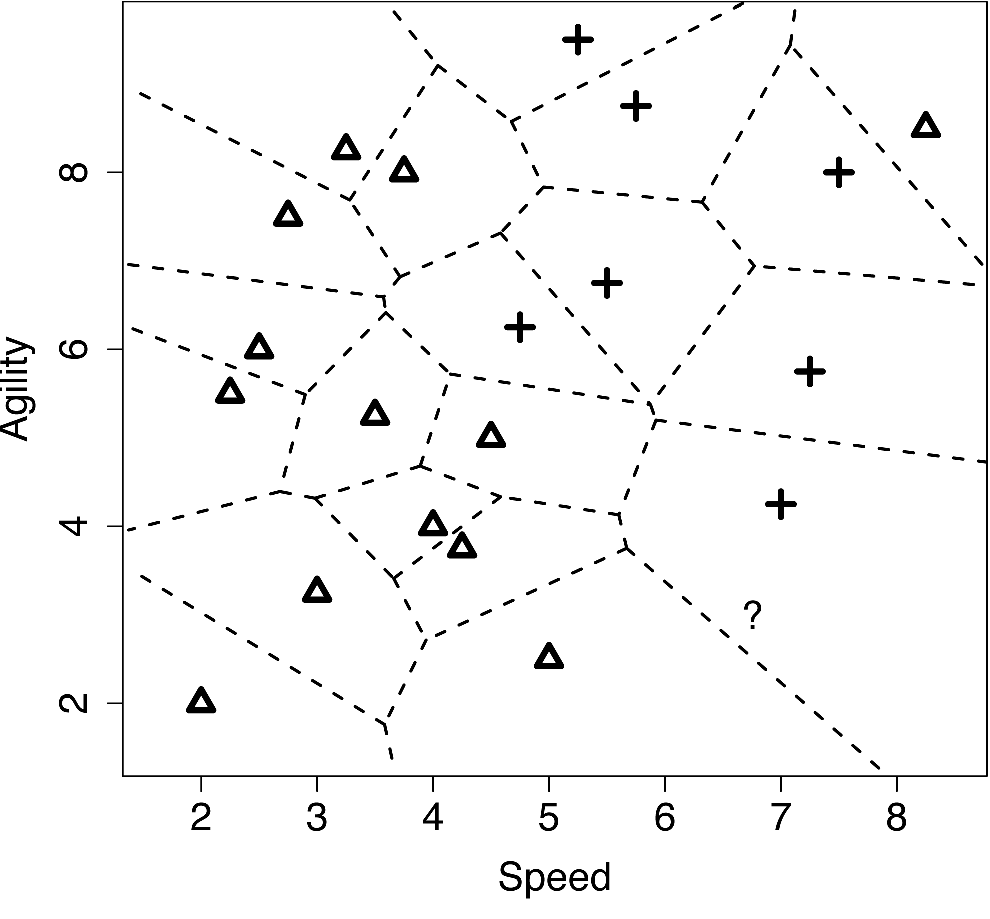
\includegraphics[width=0.47\textwidth]{./images/knn_fs_3_small.pdf}}&
\subfigure[Decision boundary ($k = 1$)]{\label{fig:voronoidecboundB}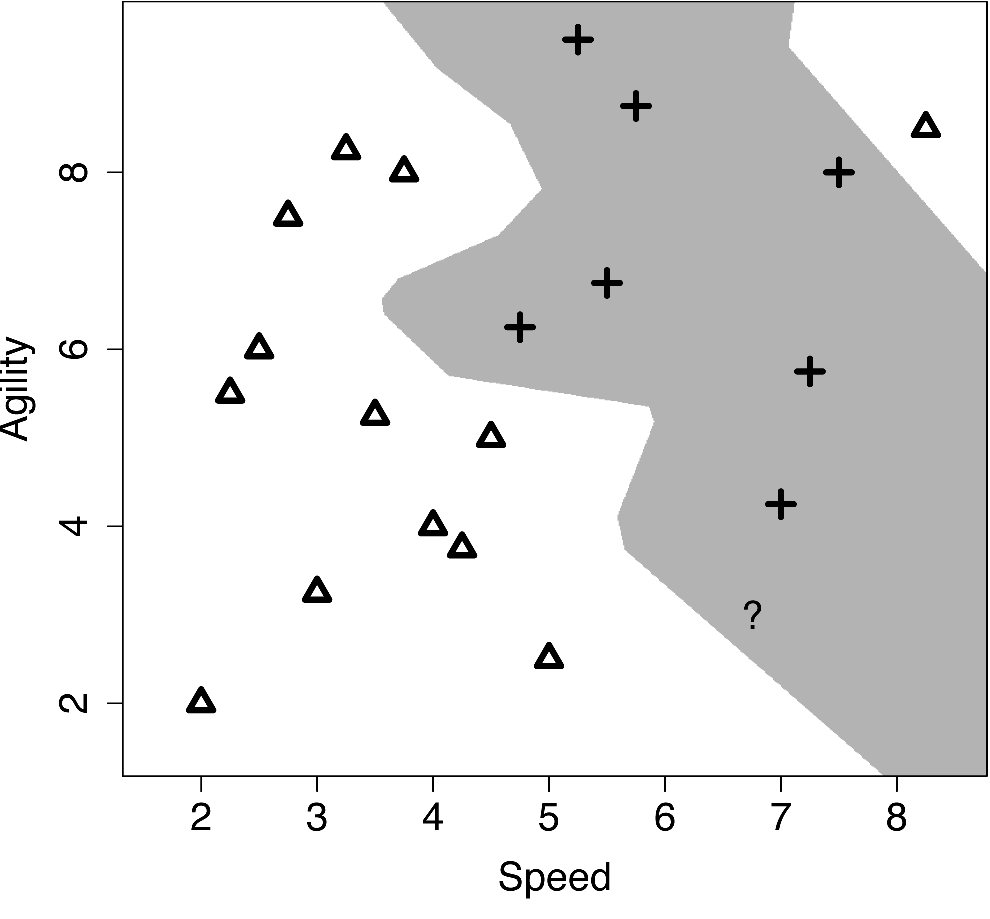
\includegraphics[width=0.47\textwidth]{./images/knn_fs_4_small.pdf}}		
	\end{tabular}
       
       \caption{(a) The Voronoi tessellation of the feature space for the dataset in Table \ourRef{table:draftProspects} with the position of the query represented by the ? marker; (b) the decision boundary created by aggregating the neighboring Voronoi regions that belong to the same target level.}	
	\label{fig:voronoidecbound}
	\end{centering}
\end{figure}
\end{frame} 

\begin{frame} 
\begin{itemize}
\item One of the great things about nearest neighbour algorithms is that we can add in new data to update the model very easily. 
\end{itemize}
\end{frame} 

 \begin{frame} 
\begin{table}[htb]
\caption{The extended version of the college athletes dataset.}
\label{table:kddataset}
\begin{scriptsize}
\begin{center}
\resizebox{\textwidth}{!}{\begin{tabular}{cc}
		\hline
			\begin{minipage}{0.41\textwidth}
				\centering
					\begin{tabular}[ht]{cccc} 
\featN{ID}	 & \featN{Speed} & \featN{Agility} & \featN{Draft}\\
\hline
1 & 2.50 & 6.00 & no\\
2 & 3.75 & 8.00 & no\\
3 & 2.25 & 5.50 & no\\
4 & 3.25 & 8.25 & no\\
5 & 2.75 & 7.50 & no\\
6 & 4.50 & 5.00 & no\\
7 & 3.50 & 5.25 & no\\
8 & 3.00 & 3.25 & no\\
9 & 4.00 & 4.00 & no\\
10 & 4.25 & 3.75 & no\\
11 & 2.00 & 2.00 & no\\
\hline
					\end{tabular}
			\end{minipage}
			&
			\begin{minipage}{0.41\textwidth}
				\centering
					\begin{tabular}[ht]{cccc} 
\featN{ID}	 & \featN{Speed} & \featN{Agility} & \featN{Draft}\\
\hline
12 & 5.00 & 2.50 & no\\
13 & 8.25 & 8.50 & no\\
14 & 5.75 & 8.75 & yes\\
15 & 4.75 & 6.25 & yes\\
16 & 5.50 & 6.75 & yes\\
17 & 5.25 & 9.50 & yes\\
18 & 7.00 & 4.25 & yes\\
19 & 7.50 & 8.00 & yes\\
20 & 7.25 & 5.75 & yes\\
21 & 6.75 & 3.00 & yes\\
~& ~ & ~ & ~\\
\hline
				\end{tabular}
			\end{minipage}\\
\end{tabular}
}
\end{center}
\end{scriptsize}
\end{table}
\end{frame} 



 \begin{frame} 
\begin{figure}[htb]
	\begin{centering}
\begin{tabular}{cc}
\subfigure[Voronoi tessellation]{\label{fig:updatedvordecA}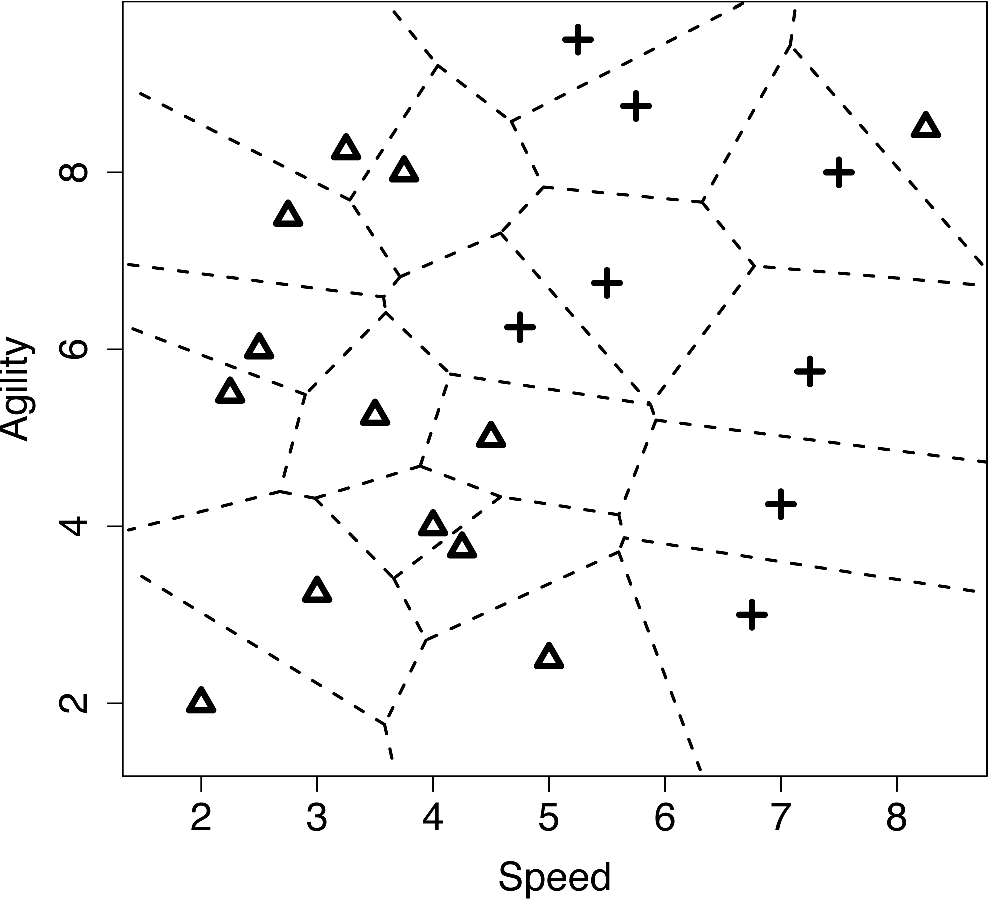
\includegraphics[width=0.47\textwidth]{./images/knn_fs_5_small.pdf}}&
\subfigure[Decision boundary ($k\,=\,1$)]{\label{fig:updatedvordecB}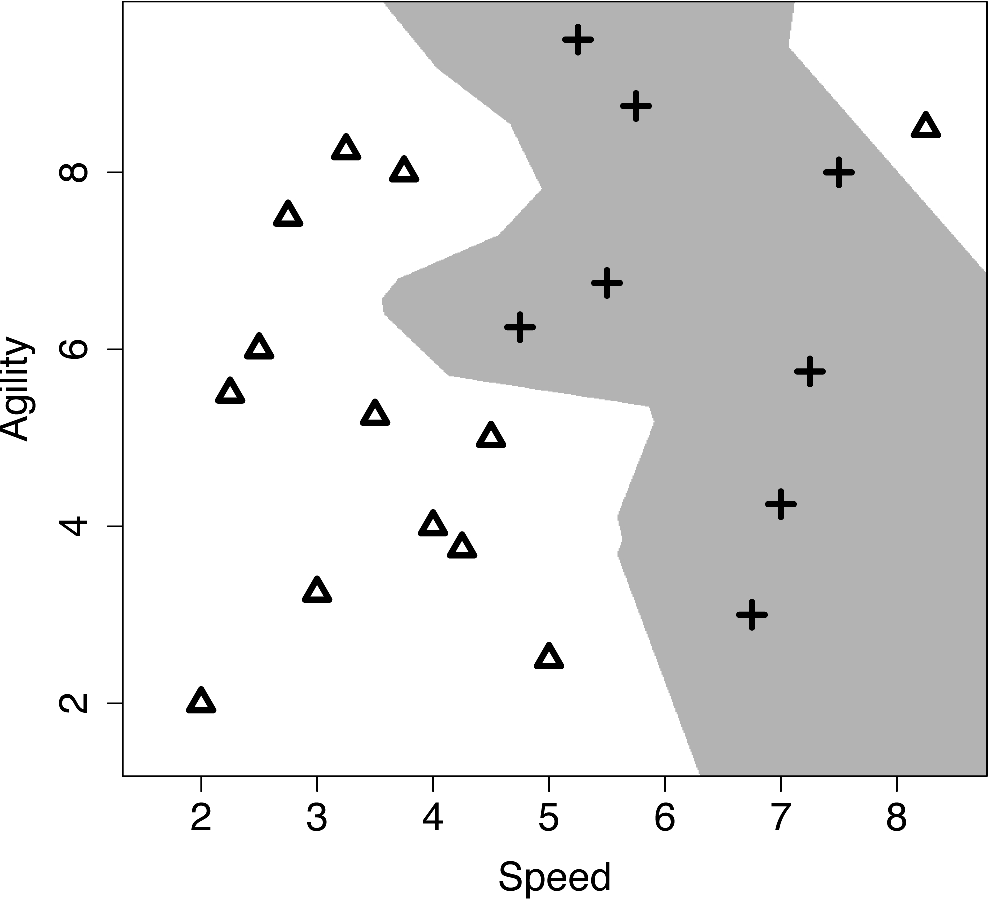
\includegraphics[width=0.47\textwidth]{./images/knn_fs_6_small.pdf}}		
	\end{tabular}
       \caption{(a) The Voronoi tessellation of the feature space when the dataset has been updated to include the query instance; (b) the updated decision boundary reflecting the addition of the query instance in the training set.}	
	\label{fig:updatedvordec}
	\end{centering}
\end{figure}
\end{frame} 

\SectionSlideShortHeader{Epilogue}{Epilogue}

\begin{frame}
\begin{itemize}
\item Returning to 1798 and HMS Calcutta, the next day you accompany your men on the expedition up the river and you encounter the strange animal the sailor had described to you. 
\item This time when you see the animal yourself you realize that it definitely isn't a duck! 
\item It turns out that you and your men are the first Europeans to encounter a platypus\footnote{The story recounted here of the discovery of the platypus is loosely based on real events.}. 
\end{itemize}
\end{frame}


 \begin{frame} 
\begin{figure}
	\begin{center}
	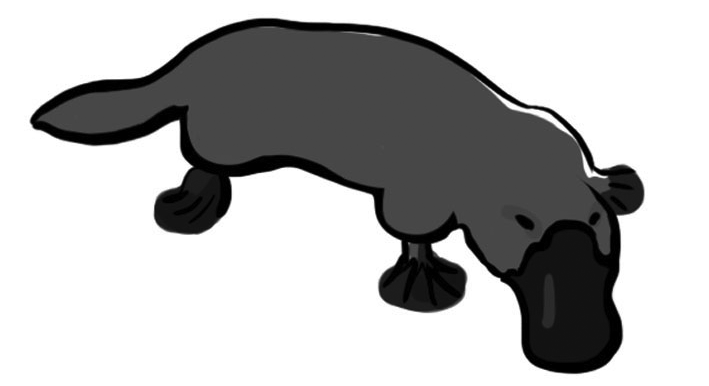
\includegraphics[width=0.4\textwidth]{./images/PlatypusBW.png}
	\end{center}
	\caption{A duck-billed platypus.The platypus image used in here was created by Jan Gillbank for the English for the Australian Curriculum website (\url{http://www.e4ac.edu.au}) and are used under the Create Commons Attribution 3.0 Unported licence (\url{http://creativecommons.org/licenses/by/3.0}). The image was sourced via Wikimedia Commons.}
	\label{fig:platypus}
\end{figure}
\end{frame} 

\begin{frame}
\begin{itemize}
\item This epilogue illustrates two important, and related, aspects of supervised machine learning:
\begin{enumerate}
	\item supervised machine learning is based on the \alert{stationarity assumption} which states that the data doesn't change - remains stationary - over time. 
	\item in the context of classification, supervised machine learning creates models that distinguish between the classes that are present in the dataset they are induced from. So, if a classification model is trained to distinguish between lions, frogs and ducks, the model will classify a query as being either a lion, a frog or a duck; even if the query is actually a platypus.
\end{enumerate}

\end{itemize} 
\end{frame} 

\SectionSlide{Summary}

\begin{frame}
\begin{itemize}
\item Similarity-based prediction models attempt to mimic a very human way of reasoning by basing predictions for a  target feature value on the most similar instances in memory---this makes them easy to interpret and understand. 
\item This advantage should not be underestimated as being able to understand how the model works gives people more confidence in the model and, hence, in the insight that it provides.
\end{itemize}
\end{frame}

\begin{frame}
\begin{itemize}
\item The inductive bias underpinning similarity-based classification is that things that are similar (i.e., instances that have similar descriptive features) belong to the same class. 
\item The nearest neighbor algorithm creates an implicit global predictive model by aggregating local models, or neighborhoods.
\item The definition of these neighborhoods is based on proximity within the feature space to the labelled training instances.
\item Queries are classified using the label of the training instance defining the neighborhood in the feature space that contains the query.  
\end{itemize}
\end{frame}


\begin{frame}
	\tableofcontents
\end{frame}



\end{document}
